\documentclass[a4paper,12pt]{article}
\usepackage{graphicx}
\usepackage{amsmath}

\def\rubik{rubik$_{2^3}$}
%%%%%%%%%%%%%%%%%%%%%%%%%%%%%%%%%%%%%%%%%%%%%%%%%%%%%%%%%%%%%%%%%%%%%%
\begin{document}
\title{\Huge \rubik\\
{\normalsize A program to compute all moves of the Rubik's pocket cube}\vspace{3em}
}
\author{Alejandro Lorca}
\date{\today}
\maketitle

\section{Installation}

If you had experience with this kind of software, issuing the commands
\begin{verbatim}
./configure
make
\end{verbatim}
do the job.
\section{Understanding the notation}
The pocket cube, contrary to the standard cube, does not have a center
facet in each face that can be used for labelling the orientation and
therefore establishing a coordinate system. 

One is free to choose a corner, from now on the {\sl reference
  corner}, place it into a given position and fix also its
orientation. This operation defines acoordinate system and permits
only moves in the opposite faces of this cublet.

\begin{figure}[!ht]
\begin{center}
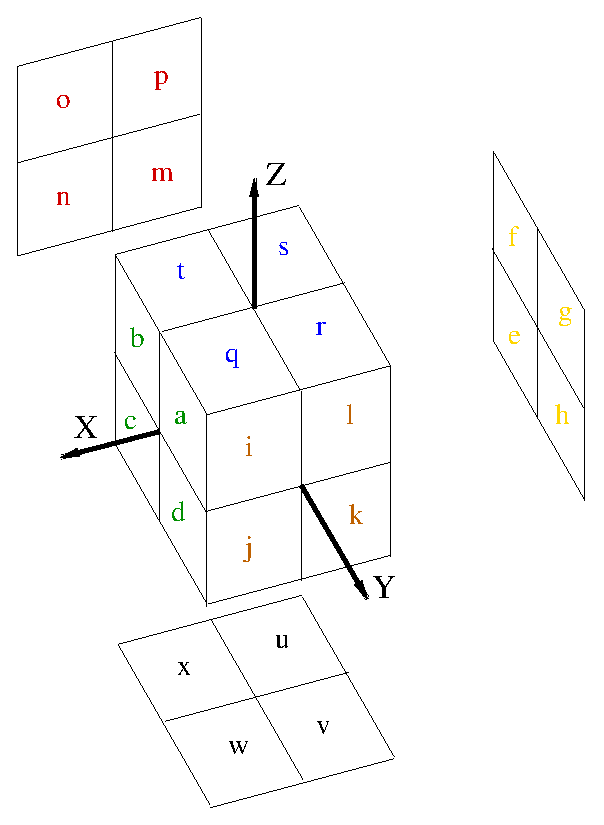
\includegraphics{notation}
\end{center}
\caption{Notation for the cube. In capital letters $X$, $Y$ and $Z$ the rotations on the opposite
  sides to the reference cublet $emu$.}
\label{notation}
\end{figure}

We will denote by $+X$,  $+Y$ and $+Z$ the operations turning a quarter
of an opposite face following anticlockwise any of the directions $x$, $y$
and $z$ (to be identified with given colors of the reference cublet).

The facets of the pocket cube will be named with characters from $a$
till $x$, following also anticlockwise conventions and beggining from
the corresponding rotation $+X$ in such a way that applying $+X$ to
the cube moves the facets in the following order
\begin{equation}
a \rightarrow b, b \rightarrow c, c \rightarrow d, d \rightarrow a.
\end{equation}

Such permutation can be written in a shorthand notation like
\begin{equation}
(abcd).
\end{equation}

As the reader has probably realized, the move $+X$ also involve facet
displacement on front and top the cube in Fig.\ref{notation}. The complete basic
one-directional quarter-turn permutations will be
\begin{align}
+X &=(abcd)(itnw)(jqox)\\
+Y &=(awhr)(dvgq)(ijkl)\\
+Z &=(alfo)(bigp)(qrst)
\end{align}




\end{document}
